% Options for packages loaded elsewhere
\PassOptionsToPackage{unicode}{hyperref}
\PassOptionsToPackage{hyphens}{url}
\documentclass[
  tikz=true]{standalone}
\usepackage{xcolor}
\usepackage{amsmath,amssymb}
\setcounter{secnumdepth}{-\maxdimen} % remove section numbering
\usepackage{iftex}
\ifPDFTeX
  \usepackage[T1]{fontenc}
  \usepackage[utf8]{inputenc}
  \usepackage{textcomp} % provide euro and other symbols
\else % if luatex or xetex
  \usepackage{unicode-math} % this also loads fontspec
  \defaultfontfeatures{Scale=MatchLowercase}
  \defaultfontfeatures[\rmfamily]{Ligatures=TeX,Scale=1}
\fi
\usepackage{lmodern}
\ifPDFTeX\else
  % xetex/luatex font selection
\fi
% Use upquote if available, for straight quotes in verbatim environments
\IfFileExists{upquote.sty}{\usepackage{upquote}}{}
\IfFileExists{microtype.sty}{% use microtype if available
  \usepackage[]{microtype}
  \UseMicrotypeSet[protrusion]{basicmath} % disable protrusion for tt fonts
}{}
\makeatletter
\@ifundefined{KOMAClassName}{% if non-KOMA class
  \IfFileExists{parskip.sty}{%
    \usepackage{parskip}
  }{% else
    \setlength{\parindent}{0pt}
    \setlength{\parskip}{6pt plus 2pt minus 1pt}}
}{% if KOMA class
  \KOMAoptions{parskip=half}}
\makeatother
\usepackage{graphicx}
\makeatletter
\newsavebox\pandoc@box
\newcommand*\pandocbounded[1]{% scales image to fit in text height/width
  \sbox\pandoc@box{#1}%
  \Gscale@div\@tempa{\textheight}{\dimexpr\ht\pandoc@box+\dp\pandoc@box\relax}%
  \Gscale@div\@tempb{\linewidth}{\wd\pandoc@box}%
  \ifdim\@tempb\p@<\@tempa\p@\let\@tempa\@tempb\fi% select the smaller of both
  \ifdim\@tempa\p@<\p@\scalebox{\@tempa}{\usebox\pandoc@box}%
  \else\usebox{\pandoc@box}%
  \fi%
}
% Set default figure placement to htbp
\def\fps@figure{htbp}
\makeatother
\setlength{\emergencystretch}{3em} % prevent overfull lines
\providecommand{\tightlist}{%
  \setlength{\itemsep}{0pt}\setlength{\parskip}{0pt}}
\usepackage{tikz}
\usepackage{pgfplots}
\pgfplotsset{compat=1.18}
\usetikzlibrary{shapes, positioning, calc, decorations.markings, chains, scopes}
\newlength{\Radius}
\setlength\Radius{4em}
\usepackage{amsmath}
\usepackage{caption}
\usepackage{bookmark}
\IfFileExists{xurl.sty}{\usepackage{xurl}}{} % add URL line breaks if available
\urlstyle{same}
% fallback for those not using the hyperref driver hyperxmp:
\makeatletter
\@ifundefined{xmpquote}{\newcommand{\xmpquote}[1]{#1}}{}
\makeatother
\hypersetup{
  hidelinks,
  pdfcreator={LaTeX via pandoc}}

\author{}
\date{\vspace{-2.5em}}

\begin{document}

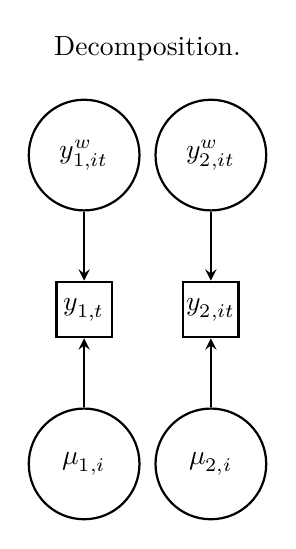
\begin{tikzpicture}[
    auto, > = latex, align=center,
    latent/.style = {
      circle, draw, thick, inner sep = 2pt, minimum width = \Radius
    },
    manifest/.style = {
      rectangle, draw, thick, inner sep = 0pt, minimum size = \Radius/2
    },
    intercept/.style = {
      regular polygon,regular polygon sides = 3, draw, thick,
      inner sep = 0pt, minimum size = \Radius
    },
    mean/.style = {
      regular polygon, regular polygon sides = 3, draw, thick,
      inner sep = 0pt, minimum size = 8mm
    },
    path/.style = {
      arrows = ->, thick, > = {stealth[]}
    },
    error/.style = {
      circle, draw = none, fill = none, thick,
      inner sep = 0pt, minimum size = 5mm
    },
    var/.style = {
      <->, thick, > = {stealth[]}, bend right = 270, looseness = 2
    },
    cov/.style = {
      <->, thick, > = {stealth[]}, bend right = 300
    },
    % style to add a circle in the middle of a path
    random/.style = {
      postaction = {
        decorate, decoration = {
          markings,
          mark = at position .5 with {
            \draw[fill = black] circle[radius = 2pt];
          }
        }
      }
    },
    random_cl/.style = {
      postaction = {decorate, decoration = {
        markings,
        mark = at position .2 with {
          \draw[fill = black] circle[radius = 2pt];}
        }
      }
    },
    ]

    % draw decomposition
    \node  [manifest]  (y1t)  {$y_{1,t}$};
    \node  [latent]  (y1wt)  [above = 2.5em of y1t]  {$y_{1,it}^w$};
    \node  [latent]  (mu1)  [below = 2.5em of y1t]  {$\mu_{1,i}$};

    % draw nodes
    \foreach \i [remember = \i as \lasti (initially 1)] in {2, ..., 2}
    \node  [manifest]  (y\i t)  [right = 2.5em of y\lasti t]  {$y_{\i,it}$};

    \foreach \i [remember = \i as \lasti (initially 1)] in {2, ..., 2}
    \node  [latent]  (y\i wt)  [above = 2.5em of y\i t]  {$y_{\i,it}^w$};

    \foreach \i [remember = \i as \lasti (initially 1)] in {2, ...,2}
    \node  [latent]  (mu\i)  [below = 2.5em of y\i t]  {$\mu_{\i,i}$};

    % draw paths
    \foreach \i [remember = \i as \lasti (initially 1)] in {1, ...,2}
    \draw  [path]  (y\i wt)  to node  []  {}  (y\i t);

    \foreach \i [remember = \i as \lasti (initially 1)] in {1, ...,2}
    \draw  [path]  (mu\i)  to node  []  {}  (y\i t);
% caption
\node  [above = 1em, align = center]  at  (current bounding box.north)  {Decomposition.};
\end{tikzpicture}
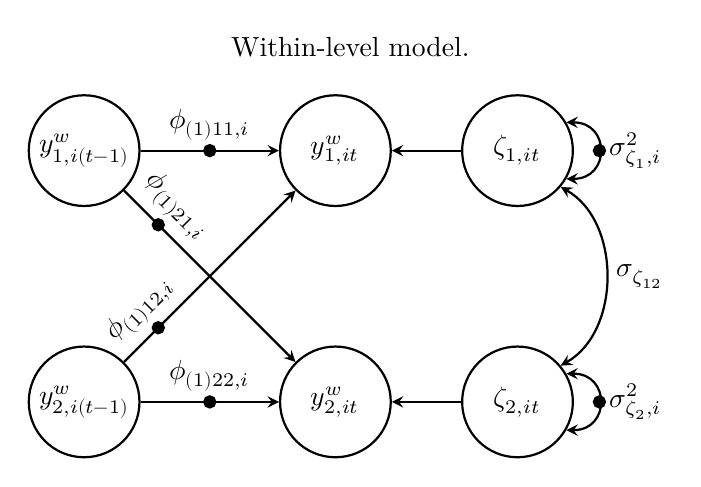
\begin{tikzpicture}[
    auto, > = latex, align=center,
    latent/.style = {
      circle, draw, thick, inner sep = 2pt, minimum width = \Radius
    },
    manifest/.style = {
      rectangle, draw, thick, inner sep = 0pt, minimum size = \Radius/2
    },
    intercept/.style = {
      regular polygon,regular polygon sides = 3, draw, thick,
      inner sep = 0pt, minimum size = \Radius
    },
    mean/.style = {
      regular polygon, regular polygon sides = 3, draw, thick,
      inner sep = 0pt, minimum size = 8mm
    },
    path/.style = {
      arrows = ->, thick, > = {stealth[]}
    },
    error/.style = {
      circle, draw = none, fill = none, thick,
      inner sep = 0pt, minimum size = 5mm
    },
    var/.style = {
      <->, thick, > = {stealth[]}, bend right = 270, looseness = 2
    },
    cov/.style = {
      <->, thick, > = {stealth[]}, bend right = 300
    },
    % style to add a circle in the middle of a path
    random/.style = {
      postaction = {
        decorate, decoration = {
          markings,
          mark = at position .5 with {
            \draw[fill = black] circle[radius = 2pt];
          }
        }
      }
    },
    random_cl/.style = {
      postaction = {decorate, decoration = {
        markings,
        mark = at position .2 with {
          \draw[fill = black] circle[radius = 2pt];}
        }
      }
    },
    ]

    % draw within-level structural model
    \node  [latent]  (y1wt-1)  {$y_{1,i(t-1)}^w$};
    \node  [latent]  (y1wt)  [right =5em of y1wt-1]  {$y_{1,it}^w$};
    \node  [latent]  (zeta1t)  [right =2.5em of y1wt]  {$\zeta_{1,it}$};

    % draw nodes
    \foreach \i [remember = \i as \lasti (initially 1)] in {2, ..., 2}
    \node  [latent]  (y\i wt-1)  [below = 5em of y\lasti wt-1]  {$y_{\i ,i(t-1)}^w$};\foreach \i [remember = \i as \lasti (initially 1)] in {2, ..., 2}
    \node  [latent]  (y\i wt)  [below = 5em of y\lasti wt]  {$y_{\i ,it}^w$};

    \foreach \i [remember = \i as \lasti (initially 1)] in {2, ..., 2}
    \node  [latent]  (zeta\i t)  [below = 5em of zeta\lasti t]  {$\zeta_{\i ,it}$};

    % draw paths from residuals to yiwt
    \foreach \i [remember = \i as \lasti (initially 1)] in {1, ...,2}
    \draw  [path]  (zeta\i t)  to node  []  {}  (y\i wt);
    
\draw  [path, postaction = random]  (y1wt-1)  to node  []  {$\phi_{(1)11,i}$}  (y1wt);
\draw  [path, postaction = random_cl, sloped, pos = .2]  (y2wt-1)  to node  []  {$\phi_{(1)12,i}$}  (y1wt);
\draw  [path, postaction = random_cl, sloped, pos = .2]  (y1wt-1)  to node  []  {$\phi_{(1)21,i}$}  (y2wt);
\draw  [path, postaction = random]  (y2wt-1)  to node  []  {$\phi_{(1)22,i}$}  (y2wt);
\draw  [var, postaction = random]  (zeta1t.30)  to node  []  {$\sigma^2_{\zeta_{1},i}$}  (zeta1t.330);
\draw  [var, postaction = random]  (zeta2t.30)  to node  []  {$\sigma^2_{\zeta_{2},i}$}  (zeta2t.330);
\draw  [cov]  (zeta1t.320)  to node  []  {$\sigma_{\zeta_{12}}$}  (zeta2t.40);
% caption
\node  [above = 1em, align = center]  at  (current bounding box.north)  {Within-level model.};
\end{tikzpicture}
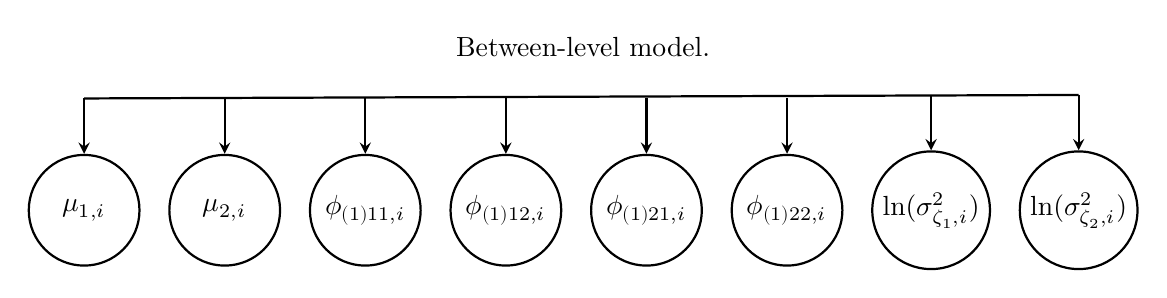
\begin{tikzpicture}[
    auto, > = latex, align=center,
    latent/.style = {
      circle, draw, thick, inner sep = 2pt, minimum width = \Radius
    },
    manifest/.style = {
      rectangle, draw, thick, inner sep = 0pt, minimum size = \Radius/2
    },
    intercept/.style = {
      regular polygon,regular polygon sides = 3, draw, thick,
      inner sep = 0pt, minimum size = \Radius
    },
    mean/.style = {
      regular polygon, regular polygon sides = 3, draw, thick,
      inner sep = 0pt, minimum size = 8mm
    },
    path/.style = {
      arrows = ->, thick, > = {stealth[]}
    },
    error/.style = {
      circle, draw = none, fill = none, thick,
      inner sep = 0pt, minimum size = 5mm
    },
    var/.style = {
      <->, thick, > = {stealth[]}, bend right = 270, looseness = 2
    },
    cov/.style = {
      <->, thick, > = {stealth[]}, bend right = 300
    },
    % style to add a circle in the middle of a path
    random/.style = {
      postaction = {
        decorate, decoration = {
          markings,
          mark = at position .5 with {
            \draw[fill = black] circle[radius = 2pt];
          }
        }
      }
    },
    random_cl/.style = {
      postaction = {decorate, decoration = {
        markings,
        mark = at position .2 with {
          \draw[fill = black] circle[radius = 2pt];}
        }
      }
    },
    ]
\node  [latent]  (mu_1)  {$\mu_{1,i}$};
\node  [latent]  (mu_2)  [right = 1em of mu_1]  {$\mu_{2,i}$};
\node  [latent]  (phi1_11)  [right = 1em of mu_2]  {$\phi_{(1)11,i}$};
\node  [latent]  (phi1_12)  [right = 1em of phi1_11]  {$\phi_{(1)12,i}$};
\node  [latent]  (phi1_21)  [right = 1em of phi1_12]  {$\phi_{(1)21,i}$};
\node  [latent]  (phi1_22)  [right = 1em of phi1_21]  {$\phi_{(1)22,i}$};
\node  [latent]  (lnsigma2_1)  [right = 1em of phi1_22]  {ln($\sigma^2_{\zeta_{1},i}$)};
\node  [latent]  (lnsigma2_2)  [right = 1em of lnsigma2_1]  {ln($\sigma^2_{\zeta_{2},i}$)};



\node  [coordinate]  (c1)  [above = 2em of mu_1]  {};
\node  [coordinate]  (c2)  [above = 2em of mu_2]  {};
\node  [coordinate]  (c3)  [above = 2em of phi1_11]  {};
\node  [coordinate]  (c4)  [above = 2em of phi1_12]  {};
\node  [coordinate]  (c5)  [above = 2em of phi1_21]  {};
\node  [coordinate]  (c6)  [above = 2em of phi1_22]  {};
\node  [coordinate]  (c7)  [above = 2em of lnsigma2_1]  {};
\node  [coordinate]  (c8)  [above = 2em of lnsigma2_2]  {}; \draw  [path]  (c1)  to node  []  {}  (mu_1);
\draw  [path]  (c2)  to node  []  {}  (mu_2);
\draw  [path]  (c3)  to node  []  {}  (phi1_11);
\draw  [path]  (c4)  to node  []  {}  (phi1_12);
\draw  [path]  (c5)  to node  []  {}  (phi1_21);
\draw  [path]  (c6)  to node  []  {}  (phi1_22);
\draw  [path]  (c7)  to node  []  {}  (lnsigma2_1);
\draw  [path]  (c8)  to node  []  {}  (lnsigma2_2); \draw  [thick]  (c1)  --  (c8);
% caption
\node  [above = 1em, align = center]  at  (current bounding box.north)  {Between-level model.};
\end{tikzpicture}

\end{document}
